\section{系统设计}
\subsection{系统设计目标和原则}
本系统旨在设计和开发一个适合少量并发,大部分局域网场景下,提供文件的上传、下载、分享、搜索、备份、视频播放等功能,
并且使这些功能在实现后易于上手使用,运行稳定并且具有良好的用户经验和可靠的安全性。 因此在设计系统中过程中必须遵循以下原则:
\par 符合开发规范:遵循系统开发各项相关标准和体系。
\par 选用成熟技术方案:为了保证开发效率和开发质量,成熟的技术方案可以保证系统的稳定性和低学习成本,因为网上的资料会比较多。
\par 完善的功能:在需求分析阶段提出的功能尽量完成,为用户提供可行的解决方案。
\par 可扩展性强:系统开发时长期的过程,需求也是不断发生变化,因此设计的时候尽量采用设计模式,预留接口,二次开发才能高效进行。
\par 维护简单:系统需要长期稳定运行,而长期稳定的运行离不开日常的维护。
\par 界面简洁,功能易用。

\subsection{服务器设计}
本云盘系统的服务器设计采用经典的LAMP架构,处理一次客户端动态资源请求的过程如图\ref{lamp_server}
所示,
\paragraph{服务器处理流程} $\mathbb{}$ $\mathbb{}$
\par a) Client发起http请求
\par b) Httpd Server Apache接收请求并交给CGI进程处理
\par c) 通过CGI接口访问PHP的的应用程序
\par d) PHP应用程序调用PHP解释器执行PHP代码
\par e) PHP程序通过Mysql驱动访问数据库数据
\par f) PHP对数据进行封装,最后给客户返回相应
\par 故在LAMP的环境机构中,apache、mariadb和php的主要功能分别如下。

\paragraph{apache主要实现如下功能:} $\mathbb{}$ $\mathbb{}$
\par a) 处理http的请求、构建响应报文等自身服务;
\par b) 配置让Apache支持PHP程序的响应,修改apache conf目录下的httpd.conf配置文件,引入PHP模块;
\par c) 配置Apache具体处理php程序的方法,在本系统中统一使用路由表来出来方法和路径映射;
\paragraph{mariadb主要实现如下功能:} $\mathbb{}$ $\mathbb{}$
\par a) 提供PHP程序对Mysql数据库数据的写入;
\par b) 提供PHP程序对Mysql数据库数据的读取;
\par c) 通常情况下从性能的角度考虑,尽量实现数据库的读写分离,但是本系统地位是个人的云盘系统,因此并发场景不多,所以没有实现读写分离
\begin{figure}[H]
    \centering
    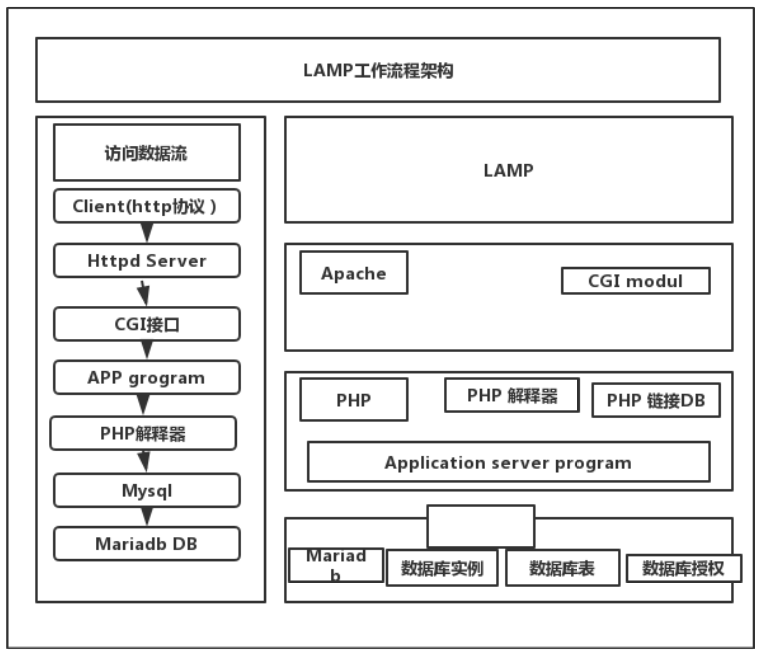
\includegraphics[width=130mm]{./figures/lamp4.png}
    \caption{LAMP架构图}
    \label{lamp_server}
\end{figure}
\paragraph{php主要实现如下功能:} $\mathbb{}$ $\mathbb{}$
\par a) 实现Apache的访问接口CGI,一般用户请求都交给CGI处理,相当于Tomcat中的servlet方法。对于Apache对静态资源的访问可以不经过CGI接口;
\par b) 提供PHP程序的解释器;
\par c) 提供Mysql数据库的访问驱动,驱动是为了将数据库的磁盘比特转化成PHP可以识别的数据结构。

具体的服务器设计如图\ref{server_img}所示。经过路由器端口映射,客户端可以在外网或者局域网的网络环境下访问服务器,在服务端,系统实现了动静资源的分离,如果是直接访问文件,直接经过
apache的路径就可以不需要php来处理请求了,直接返回静态文件资源。同时系统会添加新进程,进行文件的增量备份和异地备份。

\begin{figure}[H]
    \centering
    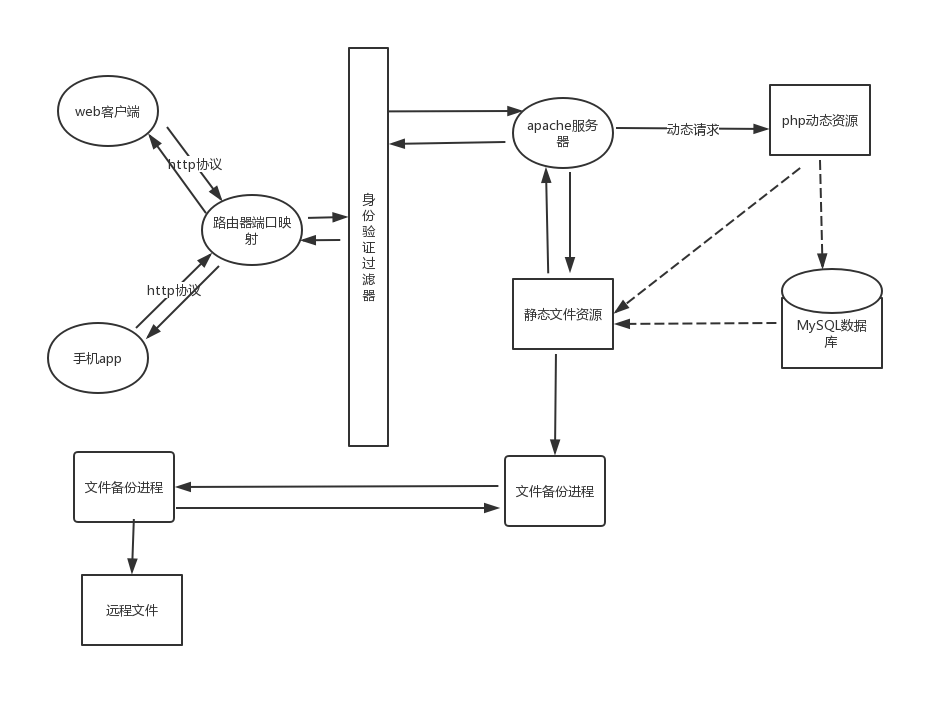
\includegraphics[width=130mm]{./figures/server.png}
    \label{server_img}
    \caption{系统总架构图}
  \end{figure}

\subsection{数据库设计}
根据系统的各个功能模块的划分和各个系统角色的从属关系,设计了一下的数据库系统,第一部分是从全局的视角展示各个系统角色之间的关系,
接下来再详细地介绍各个表字段的含义。

本文的系统数据库表格设计主要分为3个模块,分为用户模块、文件模块、系统配置模块。用户模块和文件模块有依赖关系,
系统配置模块需要规定服务器系统的硬件配置、允许访问的外网ip、内网ip、文件根路径、存储空间大小等信息。用户模块包括OcAccount、
OcMounts、OcUsers 3张表,文件模块包括OcMinetypes、OcShare、OcFilecache、OcFileTrash、OcSystemtagObjectMapping、OcSystemtag 6张表,
配置模块包括OcAppconfig、OcAppconfigKey、OcAuthtoken、OcAuthtokenWithBLOBS 4张表。

在概念设计的基础上,可以在数据库中完成实际的建表,同时建立各个表互
相之间的外键联系。在数据库的设计过程中,需要遵循一定的设计规范,以减小
数据的冗余,提高数据访问效率。本系统选用MySql 5.7版本的数据库进行
开发,需要建立的表包含系统用户、文件类型、分享文件、垃圾文件、基本文件、
文件标签、标签文件关系映射。遵循统一化驼峰法命名原则,每个表的命
名都以Oc(Own Cloud)开头,最后部分为表名称的英文。云盘系统的核心
功能的表物理结构如表\ref{user_table} \ref{type_table} \ref{share_table} 
\ref{trash_table} \ref{file_table} \ref{tag_table} \ref{middle_table}所示。

\begin{figure}[H]
    \centering
    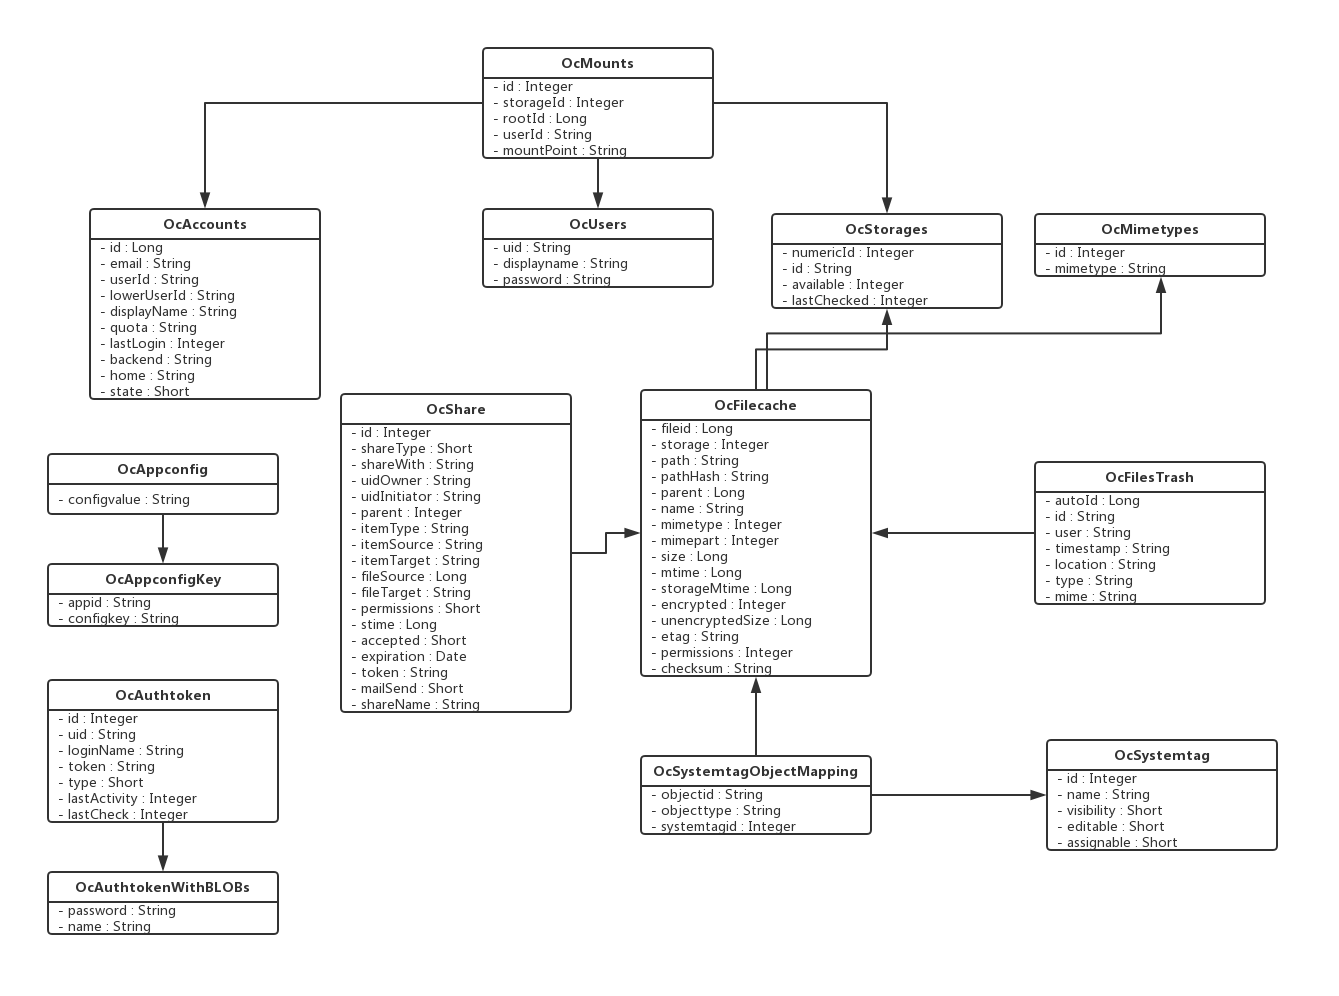
\includegraphics[width=130mm]{./figures/classes.png}
    \caption{数据库总类图}
  \end{figure}

\paragraph{用户基本信息表}
用户基本信息:包括用户id、用户昵称、口令、邮箱、存储外键、上次登录时间、家目录、用户状态。

\begin{table}[htbp]\center
    \caption{OcUsers 用户表}
    \begin{tabular}{lcccccl}
     \toprule
     字段名 & 数据类型 & 说明 \\
     \midrule
     uid         & String  &  用户id        \\
    displayname  & String  &  用户昵称      \\
    password     & String  &  口令(哈希过)\\      
    email        & String  &  邮箱          \\
    storageId    & Integer &  存储外键      \\
    lastLogin    & Integer &  上次登录时间  \\
    home         & StringA &  家目录       \\
    state        & Short   &  用户状态      \\
     \bottomrule
    \end{tabular}
    \label{user_table}    
   \end{table}

\paragraph{文件类型基本信息表}
文件类型基本信息:文件存在视频、图片、文件夹、二进制文件、可编辑文本文件、音频文件等类型
\begin{table}[htbp]\center
\caption{OcMinetypes 文件类型表}
\begin{tabular}{lcccccl}
    \toprule
    字段名 & 数据类型 & 说明 \\
    \midrule
    id         & Integer  &  id        \\
    mimetype  & String  &  文件类型      \\

    \bottomrule
\end{tabular}
\label{type_table}   
\end{table}

\paragraph{分享文件基本信息表}
分享文件基本信息:id、用户id、分享文件是文件夹类型还是文件类型、文件路径、是否允许共享、分享时间、文件身份标识、分享文件名、分享链接过期时间等

\begin{table}[htbp]\center
\caption{OcShare 分享文件表}
\begin{tabular}{lcccccl}
    \toprule
    字段名 & 数据类型 & 说明 \\
    \midrule
    id          & Integer  &   id      \\
    uid         & String   &   用户id   \\
    itemType    & String   &   文件夹或文件    \\  
    fileTarget  & String   &   文件路径     \\
    permissions & Short    &   是否允许共享\\
    stime       & Long     &   分享时间  \\
    token       & String   &   文件身份 \\     
    shareName   & String   &   分享名字  \\    
    expiration  & Date     &   过期时间   \\
    \bottomrule 
\end{tabular}
\label{share_table}   
\end{table}

\paragraph{垃圾文件信息表}
垃圾文件信息:包括id、用户id、时间戳、位置等信息。用户可把不用的文件放入垃圾箱,系统默认保存1个月的时间,在一个月时间内,用户可恢复文件,否则系统会在物理存储设备中删除文件。

\begin{table}[htbp]\center
\caption{OcFilesTrash 垃圾文件表}
\begin{tabular}{lcccccl}
    \toprule
    字段名& 数据类型 & 说明 \\
    \midrule
    id         &    String    & id   \\
    user       &    String    & 用户   \\
    timestamp  &    String    & 时间戳   \\
    location   &    String    & 位置   \\
    \bottomrule 
\end{tabular}
\label{trash_table}   
\end{table}

\paragraph{基本文件信息表}
基本文件信息: 这个表是系统的基本文件表,对文件的增删改查就是基于此表。主要包括文件id,存储,路径,路径哈希,父目录,文件名,文件类型,文件大小,上传时间,源文件创建时间,是否压缩,压缩后文件大小,文件标签,文件哈希值等信息。

\begin{table}[htbp]\center
\caption{OcFilecache 文件表}
\begin{tabular}{lcccccl}
    \toprule
    字段名& 数据类型 & 说明 \\
    \midrule
    fileid         & Long  &  文件id \\
    storage        & Integer  &  存储 \\
    path           & String  &   路径\\
    pathHash       & String  &   路径哈希\\
    parent         & Long  &   父目录\\
    name           & String  &   文件名\\
    mimetype       & Integer  &  文件类型\\
    size           & Long  &  文件大小 \\
    mtime          & Long  &  上传时间 \\
    storageMtime   & Long  &  源文件创建时间 \\
    encrypted      & Integer  &  是否压缩 \\
    unencryptedSize& Long  &   压缩后文件大小\\
    etag           & String  &  文件标签 \\
    checksum       & String  &  文件哈希值 \\
    \bottomrule 
\end{tabular}
\label{file_table}   
\end{table}

\paragraph{标签表信息表}
标签表信息:用户可以为每个文件打上标签,方便日后查找,同时用户可以为单个文件打上多个标签。主要有标签id,标签名,是否可见,是否可编辑等。

\begin{table}[htbp]\center
\caption{OcSystemtag 标签表}
\begin{tabular}{lcccccl}
    \toprule
    字段名& 数据类型 & 说明 \\
    \midrule
id          & Integer & 标签id\\
name        & String  & 标签名\\
visibility  & Short   & 是否可见\\
editable    & Short   & 是否可编辑\\
    \bottomrule 
\end{tabular}
\label{tag_table}   
\end{table}

\paragraph{标签文件中间表}
因为标签和文件之间是多对多的关系,所以需要一个中间表完成对二者关系的映射。标签文件中间表基本信息:文件id、标签id
\begin{table}[htbp]\center
\caption{OcSystemtagObjectMapping 标签文件中间表}
\begin{tabular}{lcccccl}
    \toprule
    字段名& 数据类型 & 说明 \\
    \midrule
    objectid    &  String  & 文件id\\
    systemtagid &  Integer  & 标签id\\
    \bottomrule 
\end{tabular}
\label{middle_table}   
\end{table}
\newpage